\documentclass[12pt,fleqn]{article}\usepackage{../common}
\begin{document}
Calculus'un Temel Teoremi (The Fundamental Theorem of Calculus)

Ana teoriyi ispatlamadan once iki diger teoriden bahsetmemiz, ispatlamamiz
lazim. Bu teorilerden biri Gecis Degeri Teorisi (Intermediate Value
Theorem) digeri Tanimli Entegraller Icin Ortalama Deger Teoremi (Mean Value
Theorem for Definite Integrals). Gecis Degeri Teorisi basitce sunu soyler

Teori

$[a,b]$ araliginda surekli bir fonksiyon $y=f(x)$, $f(a)$ ve $f(b)$
arasindaki her degeri muhakkak alir. Bir diger degisle, eger $y_o$, $f(a)$
ve $f(b)$ arasindaki bir deger ise $[a,b]$ araligindaki bir $c$ icin
muhakkak $y_0 = f(c)$ olmalidir. 

Geometrik olarak bu teori $y$ eksenini $f(a)$ ve $f(b)$ arasinda kesen
$y=y_0$ yatay cizgisinin $y=f(x)$ fonksiyonunu muhakkak, en az bir kez
kesecegidir. Grafik altta. 

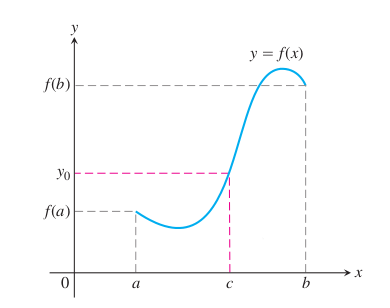
\includegraphics[height=4cm]{intermediate.png}

Sezgisel olarak bu anlamli degil mi? Eger surekli bir fonksiyon var ise,
$f(a)$'dan $f(b)$'ye giderken o araliktaki her sayiya bir kez ``ugramaya''
mecburuz. Etraflarindan dolasmamiz mumkun degil, cunku kesintili bir
fonksiyon degil, kesintisiz / surekli bir fonksiyonumuz var. Bu teorinin
daha detayli ispati icin [4]'e bakabilirsiniz. 

Maks-Min Esitsizligi

Eger $[a,b]$ araliginda $f$, maksimum deger $max \ f$'e ve minimum deger
$min \ f$'e sahipse, 

\[ min \ f \cdot (b-a) \le \int_a^b f(x)dx \le max \ f \cdot (b-a) \]

demektir. 

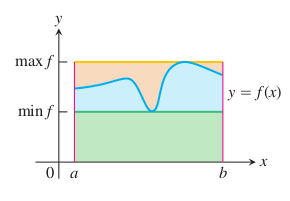
\includegraphics[height=4cm]{minmax.png}

Bu kural diyor ki $f$'in $[a,b]$ uzerindeki entegrali hicbir zaman $f$'in
minimum'u carpi $[a,b]$ araliginin uzunlugu'ndan kucuk olamaz, ve $f$'in
maksimumu carpi $[a,b]$ araliginin uzunlugu'ndan buyuk olamaz. 

Ispat

Eger $(b-a)$'yi $ \sum_{k=1}^n \Delta x_k$ olarak gorursek

\[ min \ f \cdot (b-a) = min \ f \cdot \sum_{k=1}^n \Delta x_k \]
\[  = \sum_{k=1}^n min \ f \cdot \Delta x_k  \]

$[a,b]$ araligindaki herhangi bir deger $c_k$ icin

\[  \le \sum_{k=1}^n f(c_k) \cdot \Delta x_k  \]

Oyle degil mi? $min \ f$ degeri en kucuk deger ise, $[a,b]$ araligindaki
herhangi bir nokta $c_k$'nin $f$ degeri bu degere ya esit, ya da ondan
buyuktur. Yani $min \ f \le f(c_k)$. Devam edersek

\[  \le \sum_{k=1}^n max \ f \cdot \Delta x_k  \]

Ustteki benzer mantigi takip ediyor, bu sefer $f(c_k) \le max \ f $. Son
ifadedeki $max$'i disari alabiliriz. 

\[ = max \ f \sum_{k=1}^n \cdot \Delta x_k  \]

\[ = max \ f (b-a)  \]


Ortalama Deger Teoremi

Eger $f$ fonksiyonu $[a,b]$ arasinda surekli ise o zaman $[a,b]$ araliginda
olan bir $c$ noktasinda

\[ f(c) = \frac{1}{b-a}\int_a^b f(x) dx \]

esitligi dogru olmalidir. Yani alttaki resimde sol grafikteki mavi alanin
$b-a$ ile bolunerek elde edilen ortalama degeri, $[a,b]$ araligindaki bir
$c$ uzerinden $f(c)$'ye muhakkak esittir. Ya da bir kenari $f(c)$, digeri
$b-a$ olan bir diktortgenin alani (alt sagdaki resim), mavi alanin
tamamina esit olacaktir.

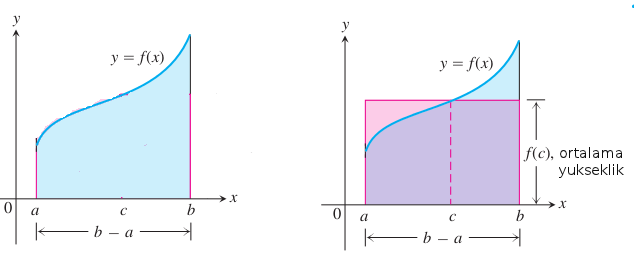
\includegraphics[height=4cm]{mean.png}

Maks-Min Esitsizliginin iki tarafini $b-a$'ya bolersek

\[ min \ f  \le \frac{1}{b-a} \int_a^b f(x)dx \le max \ f  \]

elde ederiz. Eger Gecis Degeri Teorisi dogruysa, $min \ f$ ve $max \ f$
arasindaki tum noktalar ziyaret edilmelidir. O zaman boyle bir $f(c)$
kesinlikle var demektir.

Calculus'un Temel Teoremi

Teori

Eger $f$ fonksiyonu $[a,b]$ arasinda surekli ise o zaman 

\[ F(x) = \int_a^xf(t)dt  \]

fonksiyonu da $[a,b]$ arasinda sureklidir, ve bu fonksiyonun turevi
$f(x)$'in kendisidir.

Yani

\[ F'(x) = \frac{d}{dx}\int_a^x f(t) dt = f(x)   \]

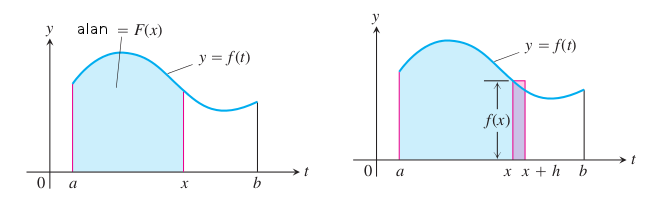
\includegraphics[height=3cm]{fund.png}

Ispat

Turevin tanimini direk $F(x)$ uzerinde uygulayalim, $[a,b]$ icinde olan $x$
ve $x+h$ araligini alalim, ve

\[ \frac{F(x+h)-F(x)}{h} \]

bolumunun limitinin, $h \to 0$ iken, $f(x)$'e gittigini gostermeye
calisalim. $F(x+h)$ ve $F(x)$ fonksiyonlarini entegralleri uzerinden
tanimlayalim. O zaman ustteki formulun bolum kismi

\[ F(x+h) - F(x) = \int_a^{x+h} f(t)dt - \int_a^x f(t)dt  \]

Entegrallerin toplam kuralina gore ustteki formulun sag tarafi 

\[ \int_x^{x+h} f(t)dt  \]

ifadesidir. O zaman bolumun tamami

\[  \frac{F(x+h)-F(x)}{h} = \frac{1}{h} \int_x^{x+h} f(t)dt   \]


Ortalama Deger Teoremine gore, ustteki esitligin sagindaki ifadenin, $x$ ve
$x+h$ araliginda $f$'in aldigi degerlerden birine aynen esit oldugunu
biliyoruz. Yani o araliktaki bir $c$ icin

\[ \frac{1}{h} \int_x^{x+h} f(t)dt = f(c) \]

kesinlikle dogru olmali. Simdi, $h \to 0$ oldukca, $x+h$ mecburen $x$'e
yaklasmak zorunda kalacaktir, cunku $c$, $x$ ile $x+h$ arasinda s�k���p
kalmistir. $f$ fonksiyonu $x$ noktasinda surekli olduguna gore, o zaman
$f(c)$, $f(x)$'e yaklasmalidir. 

\[ \lim_{h \to 0} f(c) = f(x) \]

Simdi elimizdeki bu bilgiyle basa donersek, 

\[ \frac{dF}{dx} = \lim_{h \to 0} \frac{F(x+h)-F(x)}{h} \]

\[  = \lim_{h \to 0} \frac{1}{h} \int_x^{x+h} f(t)dt   \]

\[ = \lim_{h \to 0} f(c) \]

\[ = f(x) \]


Kaynaklar

[1] Thomas Calculus 11. Baski, sf. 130

[2] Thomas Calculus 11. Baski, sf. 347

[3] Thomas Calculus 11. Baski, sf. 358

[4] Thomas Calculus 11. Baski, sf. 257


\end{document}
